\subsection{Cuellos de botellas originales, limitantes estructurales}

De las etapas descriptas en la figura \ref{fig:lio-steps}, el m\'as costoso
en la implementaci\'on existente para GPU es el paso (j). En el c\'alculo de un sistema
de tama\~no medio, este paso solo representaba el 95\% del tiempo total. Esto hacia
que esta etapa llevara tanto tiempo como todos los dem\'as c\'alculos combinados, incluso
en las GPU m\'as veloces del mercado (Tesla K40, GeForce GTX 780).

A continuaci\'on detallaremos muchos de los cambios que fueron realizados para aumentar
la performance del c\'omputo de SCF.

\subsection{Falta de accesos coalescentes}
As\'i como en CPU es importante realizar accesos alineados a memoria, en GPU es aun m\'as critico.
El termino coalescencia de memoria se define en GPU como la organizaci\'on de los accesos a memoria de secuencial, ordenada y predecible.
La l\'ogica detr\'as de esto es que cuando el GPU accede a memoria de manera alineada, puede traer entre 16 y 64 bytes en una sola lectura, suficiente para
cada uno de los threads del warp. Si en cambio debe acceder de manera no
alineada a memoria, o con threads que no acceden de manera predecible, entonces
se deber\'an serializar los accesos y separar en m\'ultiples transacciones a memoria global para satisfacer
el pedido. Este problema solamente se agrava si se debe hacer accesos frecuentes
por cientos de threads, como es el caso de los bloques con gran nivel de paralelismo explicito.

En el paso del c\'alculo de la densidades el acceso a las funciones calculadas
se realizaba por columnas en vez de por filas. Esto ocasionaba que por cada acceso,
un warp tuviera que realizar 32 accesos secuenciales a memoria, ya que no se pod\'ian alinear
en una transacci\'on. Esto, ademas, se repet\'ia para las funciones, las derivadas y los
hessianos, por lo cual los accesos eran sumamente costosos.

Para realizar el cambio de coalescencia, se tuvieron que transponer las matrices de
valores de funciones, gradientes y hessianos. La transposici\'on de matrices es un ejemplo
sumamente estudiado por la literatura de CUDA ya que ataca un punto d\'ebil de la arquitectura,
el ancho de banda de transferencia. La transposici\'on se tiene que realizar

\subsection{Subsaturacion de los SM}
La subsaturacion de los SM se da en los casos donde haya SM que est\'en listos para correr
c\'odigo pero que no puedan hacerlo porque tienen contenci\'on en algunos de sus recursos.
La m\'etrica usada para determinar esta saturaci\'on es la ocupancia de los SP.
Esta es la proporci\'on de threads activos sobre el total de threads disponibles de un bloque.

Existen en esta arquitectura principalmente tres recursos que, en un principio, parecen
ilimitados pero en realidad son finitos y compartidos por los procesadores de la GPGPU.
Estos son:
\begin{itemize}
\item Cantidad total de threads por bloque.
\item Cantidad total de registros usados por thread.
\item Cantidad de memoria compartida por bloque.
\end{itemize}

El mecanismo de scheduling de los SM funciona asignando un bloque a cada SM, que
va a correr sin preemption hasta que terminen todos sus threads asignados. Idealmente, cada
bloque cuenta con una cantidad de threads suficiente para poder esconder la latencia
de las ejecuciones mediante un cambio de contexto. La arquitectura GPGPU esta dise\~nada
para este fin, por lo cual se cuenta con un mecanismo de cambio de contexto de costo cero~\cite{NvidiaFermi} para
poder empezar a correr los threads de un warp diferente, del mismo bloque.
Si el bloque no cuenta con suficiente cantidad de threads para poner a correr de manera
concurrente, el SM va a forzosamente esperar que finalicen las operaciones de alta latencia
de estos warps sin nada que hacer mientras tanto. Si, por el contrario, se contasen con
miles de threads por bloque, entonces es posible que las operaciones que sirvan
para sincronizar los threads de todo un bloque en un punto espec\'ifico antes de proseguir
(un barrier) sean excesivamente costosas.

La arquitectura GPGPU de \nvidia organiza los registros de todos los threads en un \'unico
register file, com\'un a todos los bloques. Como cada thread usa decenas de registros para guardar
los computos intermedios, \nvidia decidi\'o unificarlos, ya que es muy variable la cantidad que va a usar
cada kernel de ejecuci\'on. Una de las grandes diferencias entre Fermi y Kepler es la cantidad m\'axima de
registros por thread. Mientras que Fermi permit\'ia hasta 63 registros, Kepler permite hasta 255. Esto
es positivo para poder correr bloques de pocos threads pero gran cantidad de registros. Por otro lado,
aumenta la presion sobre el register file. Cuando se lanzan muchos threads
que puedan estar corriendo paralelamente entre todos los SM de la GPU, es posible que se supere
la cantidad m\'axima de registros presentes en el register file. Esto fuerza a que el scheduler
no pueda poner a ejecutar m\'as bloques que los que pueda soportar este recurso, dejando SP ociosos.

Finalmente, al igual que con los registros, la memoria compartida es un recurso limitado. Como
solamente se cuenta con hasta 48Kb (Fermi-Kepler) de memoria de este tipo para ser repartida entre
todos los bloques que est\'en corriendo en todos los SM, el scheduler deber\'a decidir no poner a ejecutar
m\'as bloques simult\'aneamente que los que pueda soportar la cantidad de memoria compartida.

El problema tratado dentro de esta tesis cont\'o con todos estos limitantes. Afortunadamente,
las herramientas de profiling usadas remarca estos limitantes constantemente, haci\'endolas
fundamentales a la hora de evaluar como proseguir en la b\'usqueda de optimizaciones de c\'odigo.

\subsection{Cambios en el threading}
%Cambiamos de blocks por puntos, a blocks por funci\'on.

De los 3 kernels que originalmente compon\'ian la iteraci\'on de SCF en GPU, el que se encargaba
del c\'alculo de la densidad electr\'onica de la contribuci\'on de la energ\'ia de intercambio correlaci\'on
insum\'ia el 94\% del tiempo total de uso de la GPU. Minimizar el tiempo de ejecuci\'on de
esta funci\'on resultaba vital para poder disminuir el tiempo de convergencia de SCF.

Este kernel computa resoluci\'on num\'erica de la integral descripta en la secci\'on introductoria.
\begin{equation}
    E_{XC} = \int \rho(r) \epsilon_{xc}\left( \rho(r) \right ) dr
\end{equation}
\begin{center}
    $\Downarrow$
\end{center}
\begin{equation}
    E_{XC} \approx \sum_j \rho(r_j) \epsilon_{xc} (\rho(r_j))
\end{equation}
Esta calcula el termino de la energ\'ia de intercambio correlaci\'on, usando una grilla
de puntos con peso. Esta cuenta se realiza por cada partici\'on de los grupos en el mallado
del problema. El t\'ermino $\rho$ se obtiene de la base gaussiana usada, y $\epsilon_{xc}$
son los coeficientes variacionales. La operatoria entonces que se realiza
en el procesador es
\begin{equation}
  E_{XC} \approx \sum^{puntos} \sum_{i<m} F_i \sum_{j<i} F_j C_{i,j}
\end{equation}

Donde $F_i$, $F_j$ son los valores del mallado de las funciones de la base en un punto dado,
$m$ es la cantidad de funciones de la base y $C_{i,j}$ son los $\epsilon_{xc}$.

El cuello de botella fundamental en la ejecuci\'on radicaba en como se distribu\'ia el trabajo de computo
entre los kernels. La estrategia de paralelizaci\'on original determinaba la partici\'on
del sistema a resolver instanciando un bloque por cada punto ({$blockId.x < m$}),
una cantidad fija de threads (usando $threadId.x < BLOCK\_SIZE$)
Los threads serv\'ian para reutilizar la memoria compartida; cada thread le\'ia un
elemento de la matriz de coeficientes ($C_{i,j})$) y luego lo compart\'ian con los
dem\'as threads.

Esta distribuci\'on resultaba natural al problema, pero visto con mayor detalle, esto
implicaba una cantidad de cuentas innecesarias que pod\'ian ser eliminadas.

\begin{figure}[htbp]
   \centering
   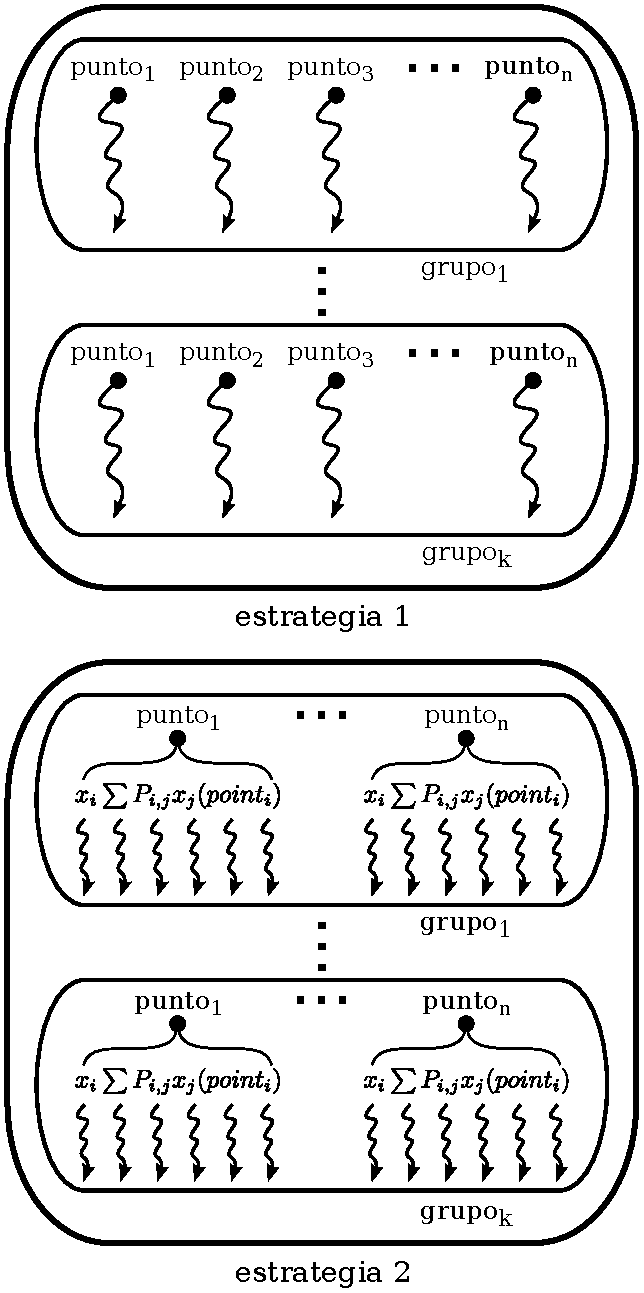
\includegraphics[width=250px]{images/cuda-parallelism.pdf}
   \caption{Estrategia original y modificada de paralelismo en el kernel de computo de la densidad
   electr\'onica computada durante $E_{XC}$.}
   \label{fig:cuda-xc-parallelism}
\end{figure}

El cambio m\'as importante para la performance provino de reconsiderar
la estrategia de partici\'on. La grilla con un bloque por punto con una cantidad
fija de threads tiene el problema de que, con bases grandes, tiene que realizar
mucho trabajo por bloque. Esto causa que los SM est\'en ocupados constantemente
por kernels de larga duraci\'on. Lo que se busca es que los  bloques realicen
menos trabajo por llamada, de modo que se puedan despachar a mas SM a medida
que estos terminen. En definitiva, lo que se busca es incrementar el throughput
de la placa. Esta estrategia se observa en la parte superior de la figura
\ref{fig:cuda-xc-parallelism}.

La nueva partici\'on que se eligi\'o dispone un bloque por funci\'on,
de modo que cada thread $i$ realice la cuenta $F_i \sum_{j}^{i} F_j C_{i,j}$
y se compartan entre threads los valores de $F_i$ le\'idos.
Esta estrategia se ve en la parte inferior de la figura \ref{fig:cuda-xc-parallelism}.

La nueva estrategia permite una mucho mayor reutilizaci\'on de las lecturas a memoria
global (uno de los grandes limitantes de esta arquitectura). Este cambio es posible ahora
dado el tama\~no de las memorias compartidas (16Kb en la generaci\'on de
dispositivos existentes en implementaci\'on original, actualmente 48Kb). Finalmente
esto tambi\'en se beneficia del incremento en tanto la cantidad de SM y la de SP por
SM. Todos estos factores permitieron una gran aceleraci\'on.

El otro cambio importantes fue partir en problema en m\'as bloques, para las grupos que tengan
m\'as funciones. Decidimos agregar otra dimensi\'on a la grilla de bloques (\texttt{blockId.y}),
para determinar cuantos grupos de threads van a hacer falta para procesar completamente
todas las funciones de ese punto. Llamamos a este par\'ametro $altura\_bloques$. Se
calcula para cada partici\'on como $altura\_bloques = {m}/{BLOCK\_SIZE}$.
Para las particiones chicas, este valor no supera a 1. En los cubos y esferas m\'as
grandes (de los sistemas probados), la altura puede ser hasta 6. Esto significa una gran
cantidad de bloques adicionales con respecto al m\'etodo anterior.

\begin{figure}[htbp]
   \centering
   \includegraphics[width=\plotwidth]{plots/cuda/threading.png}
   \caption{Speedup en veces de correr Hemoglobina en distintas arquitecturas con el cambio de estrategia}
   \label{plt:speedup-threading}
\end{figure}

%%
%%

Despu\'es de haber hecho el cambio de la paralelizaci\'on, estudiamos realizar
m\'as de un punto por thread. Esto sirve para aprovechar un par de lecturas que son comunes
entre dos funciones. Con este cambio, se instancian menos bloques (la mitad de la dimensi\'on $y$
definida para esto) y se pueden ocultar algunas latencias de acceso, pero
cada grupo de threads lleva m\'as tiempo y usan m\'as registros. Esta estrategia es similar
a un loop unrolling manual, aplicado a la arquitectura GPU.

Un punto de intensa discusi\'on durante estos cambios es el valor de \textit{BLOCK\_SIZE}.
Para nuestro problema, decidimos utilizar un numero de threads por bloque m\'ultiplo del
tama\~no de un warp (32 threads). Esto permite estudiar como afectan en el tiempo de
procesamiento contar con uno o m\'as warps por bloque. Una ventaja de usar bloques de
32 threads, es que el costo de la sincronizaci\'on es exactamente cero. No se precisa
sincronizar nada puesto que los threads trabajan en lock-step sincronizados por warp.
Un bloque chico ademas nos permite usar mas memoria compartida por thread, dado que hay una
cantidad fija de memoria por bloque (entre 32Kb y 64Kb). Cuando se cuentan con muchos m\'as
threads, se debe reducir este uso por thread de modo que todos puedan ejecutar concurrentemente.

Dicho esto, la literatura~\cite{farberCuda} sugiere siempre que sea posible
usar bloques grandes y con threads lo m\'as independientes posibles. Una gran cantidad de threads
en un bloque permite tener muchos m\'as warps para schedulear de modo de esconder las latencias de
operaciones y de a accesos globales. Sin embargo, contar con muchos threads hace que las
sincronizaciones sean mucho m\'as costosas. Ademas, como cada SM no cuenta con preemption
de bloques, contar con muchos threads por bloque hace que los recursos se mantengan
por largos periodos.

Inicialmente, este tama\~no se hab\'ia fijado en 128 threads por bloque, 4 warps. Utilizando
mas memoria compartida en el esquema de paralelizaci\'on para disminuir accesos a memoria global,
este valor resulto demasiado elevado y disminu\'ia la posibilidad de ocupar todos los SM en dispositivos
Fermi y Kepler. Con solamente 32 threads, se pod\'ia maximizar la ocupaci\'on de los SM, pero hab\'ia
muchos m\'as bloques. Finalmente, luego de disminuir un poco el uso de memoria compartida por
bloque, usando algunas ideas descriptas a continuaci\'on, pudimos fijar este valor en 64 threads
por bloque. Mostramos que tener solo un warp es bueno, pero mucho mejor a\'un es tener dos warps, porque
esto permite, con costo cero, poner a correr el otro para ocultar la latencia sin agrandar
demasiado el costo de la sincronizaci\'on.

Habiendo hechas todas las dem\'as optimizaciones detalladas en las secciones siguientes, evaluamos
\'unicamente este par\'ametro. Evaluamos un bloque de 32 threads hasta 128 threads por bloque,
el m\'aximo valor posible de modo que entre nuestro uso de memoria compartida.

\begin{figure}[htbp]
   \centering
   \includegraphics[width=\plotwidth]{plots/cuda/dbs.png}
   \caption{Speedup en veces del kernel density corriendo Hemoglobina variando
   la arquitectura y tama\~no de \textit{BLOCK\_SIZE}.}
   \label{plt:dbs-runtime}
\end{figure}


\subsection{Cambios en la reducci\'on}
%Hubo que agregar reducci\'on de suma a nivel punto porque ya no se comparten mas la info
La reorganizaci\'on de la paralelizaci\'on del kernel del calculo de la densidad creo la necesidad
de varios pasos de reducci\'on que antes se hac\'ian impl\'icitamente.

El primer paso, al ya no haber un bloque por punto, habr\'a que totalizar el c\'alculo de la
suma de todos los elementos de la columna que acabamos de procesar para obtenerlo. Para reducir,
vamos a reutilizar la memoria shared que empleamos en el c\'alculo de la energ\'ia anterior. Cada
thread va a poner el valor final del computo realizado en su posici\'on correspondiente en el
la memoria compartida. Esto luego se ejecuta como una reducci\'on en \'arbol, donde cada
thread suma el valor de la posici\'on $x$ con el valor en $2*x$, si fuera este valido. Esto
luego se repite por la mitad de los threads, hasta que solo el thread 0 lo ejecuta,
generando exactamente un valor por bloque, que lo va a terminar escribiendo en la memoria
global.

Esta t\'ecnica de reducci\'on es sumamente conocida para arquitecturas distribuidas, generando
la respuesta en $O(log_2(n))$ pasos. La literatura de CUDA~\cite{cudaReductions} sugiere t\'ecnicas adicionales para
minimizar a\'un mas el tiempo empleado en esta reducci\'on, pero considerando que hay, a lo sumo
6 operaciones, no hay necesidad de mejorar esto mas.

Como va a haber $altura\_{bloque}$ cantidad de escrituras para cada punto, va a entonces
hacer falta guardar estas cuentas parciales en memoria global. Para eso definimos una matriz
por cada uno de los par\'ametros que debemos acumular, con tama\~no id\'entico a la cantidad de bloques
del kernel \texttt{compute\_energy}, para que cada uno de estos escriba \'unicamente en una posici\'on
un\'ivocamente identificada de este. Estas matrices luego son de tama\~no $O(\#_{puntos} * altura_{bloque})$,
menos de 1Mb en el caso m\'as grande.

El siguiente paso de la reducci\'on consiste en acumular los $altura\_{bloque}$ valores descriptos
reci\'en en un solo por punto. Esto implica encontrar donde est\'an en las matrices temporales las
partes de las cuentas, agregarlas y calcular el potencial correcto. Esto genera finalmente los
coeficientes para calcular la actualizaci\'on de la matriz de Kohn-Sham y los factores para el
c\'alculo de la matriz de fuerzas.

Esto se refleja en el c\'odigo como una llamada a un nuevo kernel adicional, posterior a la
cuenta de la densidad y con m\'ultiples matrices temporales adicionales. Este kernel es sumamente
eficiente porque ya todo el trabajo pesado lo hizo el anterior. Solo se tiene que realizar
a lo sumo $altura\_{bloque}$ sumas y una llamada a la funci\'on que calcula el potencial y densidad,
un kernel corto de alta intensidad aritm\'etica que realiza solamente operaciones matem\'aticas.
Finalmente, la acumulaci\'on finaliza, generando un valor por cada punto, lo mismo que se produc\'ia
anteriormente pero utilizando mucho mejor los recursos del dispositivo.


%%%%%%%%%%%%%%%5


\subsection{Cambios en los accesos globales}
La arquitectura de las placas de v\'ideo est\'an pensadas entorno al poder de computo.
Las decisiones tomadas por los dise\~nadores de las GPGPU se concentran alrededor
de paralelismo a lo ancho, poniendo un gran \'enfasis en la cantidad de n\'ucleos. Luego,
se dispone de menor cantidad de espacio disponible en el \textit{die} para las memorias.

Esta decisi\'on implica que la amplia mayor\'ia de la memoria de la GPGPU se encuentra
localizada externa al procesador.  No solo esta f\'isicamente mas lejos, sino que
adem\'as la latencia para accederla es muy elevada. Es decir, el paradigma de
programaci\'on de las GPGPU gira entorno a esconder la gran latencia de los accesos
a las memorias globales.

Una de las memorias intermedias entre entre el procesador y la memoria global es
la memoria de textura. La memoria de textura es un cach\'e sobre la memoria global,
que esta focalizado alrededor de los accesos a memoria en varias dimensiones.
Estas memorias reciben su nombre de su funci\'on principal, que es en el \'area de los
sistemas de v\'ideo. Los mapas de textura suelen ser grandes matrices que definen
tanto los colores sobre las superficies de los pol\'igonos como los relieves.
El detalle crucial de estas memorias es que un miss en estas cache, provoca
que se traigan datos no solo contiguos en memoria, como pasa en las caches de
CPU normalmente, sino que ademas se traigan los datos en posiciones l\'ogicas contiguas,
es decir, variando las distintas dimensiones de la matriz subyacente.

Las memorias de textura se ajustan bien a los problemas de GPGPU, porque se relacionan
\'intimamente con los los mecanismos de paralelismo de CUDA. Como los problemas se pueden
dividir en bloques con threads en $x$, $y$, $z$, entonces tiene mucho sentido pensar
que las estructuras de datos subyacentes se van a acceder usando indices multidimensionales.

En nuestro problema, la memoria de textura se presenta como una soluci\'on para
los accesos bidimensionales de la matriz de coeficientes para el grupo de puntos.
Como esta matriz debe ser multiplicada por todos los valores de las funciones,
derivadas primeras y segundas, se va a acceder a toda la matriz de coeficientes mas de
una vez por cada thread. Adem\'as, como se va a usar toda la matriz, y esta suele
tener un tama\~no intermedio (es muy grande para memoria constante), el problema
suele entrar casi completamente en la memoria de textura.
La lectura bidimensional en este caso, se ajusta muy bien a los accesos por filas
y por columnas a la matriz.

\begin{figure}[htbp]
   \centering
   \includegraphics[width=\plotwidth]{plots/cuda/texture.png}
   \caption{Aceleracion del c\'alculo de densidad corriendo Hemoglobina en Fermi y Kepler
   usando memoria de textura para leer los coeficientes variacionales.}
   \label{plt:texture}
\end{figure}

Como podemos ver en la figura~\ref{plt:texture}, esta optimizaci\'on aprovecha este
recurso \'unico de GPU. Sin embargo, esto agrega un factor mas que tenemos que tener en
cuenta a la hora de profilear el c\'odigo. Para administrar los accesos a
la memoria de textura, cada multiprocesador tiene m\'ultiples unidades de textura.
Cuando dependemos de sobremanera de la memoria de textura para esconder la latencia,
se presentan contenciones sobre el acceso a estas unidades. Esta cach\'e hay que usarla
solamente en los accesos mas costosos únicamente, ya que si intentamos pasar todos
los accesos a través de este, no solo no se verían mejoras, sino que seria un retroceso
completo de performance, como sucedió cuando se intent\'o agregar adem\'as las matrices
de funciones a este m\'etodo.

%http://www.realworldtech.com/gt200/10/   << detalles sobre texture cache invalidation

%\subsection{Cambios en los pasajes de informaci\'on intrawarp}
%%Los shuffles que no anduvieron salvo en function
%La arquitectura SM35, junto con CUDA5, trajeron aparejadas una herramienta interesante
%para el manejo interno de los pasajes de informaci\'on intra-warp durante la ejecuci\'on.
%Las instrucciones de shuffle, como asi las denomina \nvidia, son instrucciones que facilitan
%el pasaje directo de un registro de un thread en un warp, a otro, en un solo ciclo de ejecuci\'on.
%Estas instrucciones existen en diversas maneras, con distintos propositos. Principalmente se
%utilizan para pasar de un thread al siguiente (modulo el warp size) un registro para poder seguir
%operando. Otro uso que puede tener mucho interes proximamente son las instrucciones de votaci\'on,
%donde se evalua un predicado para todos los threads, y se setea o limpia un bit en el resultado
%de respuesta si se cumplio el predicado para ese thread. Con esta herramienta, no es necesario
%acceder a memoria compartida para poder pasar minima informaci\'on dentro de cada warp.
%
%Nuestro uso de las funci\'ones de shuffle consistio en intentar eliminar lo m\'as que podiamos
%los accesos a la memoria compartida, una fuente de bloqueos porque, a pesar de que ya corre
%todos los bloques concurrentemente, leer elementos de ahi toman 4 ciclos en vez de uno solo
%como en las funci\'ones de shuffle.
%
%Probamos pasar de a un elemento y de a uno o dos vectores de 3 elementos, para comparar
%cuan notable era el impacto del acceso mas veloz.
%
%Finalmente concluimos que era una opcion valida para el pasaje de los valores de la funci\'on,
%pero que el overhead de uso para cosas como los hessianos de la funci\'on no justifica el uso.
%Adem\'as, como estas funci\'ones de shuffle solo estan presentes en las ultimas placas Kepler,
%consideramos que el aprovechamiento marginal de los recursos no era lo suficientemente meritorio
%de romper compatibilidad con las placas de la generacion Fermi anterior.


\subsection{Cambios en el almacenamiento de matrices temporales}
Una de las principales limitaciones de las GPGPU es la cantidad fija de memoria. Esta no es
expandible dado que esta soldada a la placa. Esto era aun m\'as notorio cuando las placas
contaban con menos de 1Gb de memoria (A\~nos 2007-2008).
Para problemas de calculo num\'erico, esto era un limitante muy serio; los problemas que
normalmente entraban en la memoria principal de un CPU, no entraban completos en las GPU.
La decisi\'on tomada por muchas aplicaciones de entonces es compensar esto calculando
datos intermedios y tir\'andolos al final; teniendo que ser recalculados en las pr\'oximas iteraciones.

Esta estrategia es claramente impr\'actica en CPU, puesto que se cuenta con mucha m\'as memoria
de uso general. En GPU era necesario por el faltante de memoria, pero puesto que estas cuentas se pueden
hacer m\'as r\'apido que en CPU, convirti\'endose entonces en una estrategia valida.

Cuando la aplicaci\'on original se concibi\'o, no hab\'ia siquiera placas GPGPU apuntadas a HPC, con
m\'as memoria disponible que los modelos de consumidores. Aprovechando estos recursos actuales,
desarrollamos un m\'etodos para poder almacenar las matrices de los valores de funciones y sus derivadas
en cada punto para cada grupo durante la ejecuci\'on de la aplicaci\'on, de modo de poder aprovechar
este recurso que originalmente era limitante pero ya no. Estas incluyen la matriz de funciones,
con una cantidad de elementos $O(puntos \times funciones)$, y si se usa el m\'etodo GGA
(\textit{Generalized Gradient Approximation}) para realizar los c\'alculos de DFT, tambi\'en se requieren
las matrices de gradientes y hessianos de las funciones ($O(3 \times puntos \times funciones)$ y
$O(6 \times puntos \times funciones)$ respectivamente).

Para poder determinar que cosas van a ser guardadas en memoria y que no, se determin\'o una heur\'istica
que define el orden de las particiones a solucionar. Esta heur\'istica estima que tama\~no van a
tener las matrices temporales a almacenar y ordena las particiones de menor a mayor. Esto
esta basado en el criterio de que, si bien es proporcional el tiempo de computo de estas matrices
temporales a la cantidad de funciones por grupo y cantidad de puntos (lo que determina el tama\~no
de la partici\'on), la constante es elevada. Determinamos entonces que es m\'as conveniente
aprovechar la memoria de la placa que almacena muchas matrices temporales de particiones chicas
a que almacene solamente un par de las grandes.

Para controlar la administraci\'on de memoria, se calcula si la placa dispone
con la suficiente memoria libre para guardar las matrices de funciones, y si puede, se almacenan de manera
permanente (hasta que la partici\'on se mueva a otro dispositivo o la liberaci\'on de recursos al
finalizar las iteraciones de SCF). Este mecanismo adem\'as es configurable de modo que una ejecuci\'on
pueda usar un porcentaje de la memoria con la que cuenta la placa, para poder correr m\'ultiples procesos de
simulaci\'on concurrentemente.

Un detalle a tener en cuenta es que, incluso si se maximiza el porcentaje de memoria usado para
cachear estas matrices, tal vez no alcanza para que quepa todo el sistema evaluado en memoria. Esto
se nota principalmente en la linea GeForce, que cuentan con aproximadamente entre un cuarto y la mitad
de la memoria global que tienen su equivalente en la linea Tesla. Esto es mitigado cuando se computa
m\'ultiples placas, que tambi\'en distribuyen el almacenamiento ademas del computo.

Evaluamos el tiempo de ejecuci\'on de un sistema modelando un fullereno $C_{60}$, variando la
cantidad de memoria disponible para el cacheo.

\begin{figure}[htbp]
   \centering
   \includegraphics[width=\plotwidth]{plots/cuda/global-fullereno.png}
   \caption{Aceleraci\'on del c\'alculo de una iteraci\'on de SCF en funci\'on de la memoria libre de
   la placa usada para almacenar las funciones, entre 0 y 4240 Mb.}
   \label{plt:global-fullereno}
\end{figure}


\begin{figure}[htbp]
   \centering
   \includegraphics[width=\plotwidth]{plots/cuda/global-detailed-fullereno.png}
   \caption{Aceleraci\'on del c\'alculo de una iteraci\'on de SCF en funci\'on de la memoria libre de
   la placa usada para almacenar las funciones, entre 0 y 530 Mb.}
   \label{plt:global-detailed-fullereno}
\end{figure}

Como se puede ver en las figuras \ref{plt:global-fullereno} y \ref{plt:global-detailed-fullereno}, el
uso de el almacenamiento de las funciones produce una mejora de hasta el 25\% en el tiempo de ejecuci\'on
de toda una iteraci\'on de SCF. Es muy interesante notar que son los primeros grupos los que causan mayor
diferencia en los tiempos de ejecuci\'on. Con 5.3 Mb, se pueden guardar los 23 grupos mas peque\~nos del
fullereno $C_{60}$  y de ah\'i en m\'as, el impacto de la mejora decae. Esto es as\'i porque en grupos
chicos, el overhead del c\'alculo usando kernel de funciones es muy elevado en comparaci\'on a las
cuentas (se desperdician muchos threads). Este comportamiento se puede ver
bien en en la figura~\ref{plt:runtime-functions-fullereno}, donde se puede apreciar el importante
peso de los grupos chicos en el tiempo total del calculo de las funciones. Decidimos no intentar
optimizar el c\'alculo ya que al almacenar las matrices este costo directamente se hace cero para
casi todos los grupos (dependiendo si el sistema entra entero o no en memoria).

\begin{figure}[htbp]
   \centering
   \includegraphics[width=\plotwidth]{plots/cuda/global-functions-acc.png}
   \caption{Acumulado del runtime del calculo de las funciones de los grupos ordenados
     por tama\~no de las matrices de funciones en funci\'on del tama\~no acumulado de estas,
     en un Fullereno $C_{60}$.}
   \label{plt:runtime-functions-fullereno}
\end{figure}

Esta simple mejora permite explotar el hecho de que las placas hayan aumentado dram\'aticamente su
capacidad de almacenamiento, un recurso que hasta recientemente venia siendo un limitante podemos
convertirlo en una aceleraci\'on notoria.

\subsection{Cambios en las memorias compartidas}
%Cambiar los vec\_type4 por 3 en los accesos a la shared es mucho mejor, no hace falta alinear ahi
Otro de los problemas existentes del c\'odigo que quisimos atacar fue el mejor empleo de las
memorias shared. Estas son un recurso finito y muy importante, ya que son un limitante de
la ocupancia de los multiprocesadores. Como pueden correr una cantidad de bloques que, a lo sumo,
no superen los 48Kb de memoria shared simult\'aneamente entre todos, es imprescindible minimizar el
alocacion de la memoria shared de modo que no estemos subutilizando los SM.

Una cosa que probamos, con un grado de \'exito variable, fue disminuir el tama\~no de los vectores
donde almacenamos las derivadas direccionales. Como nuestro problema es en tres dimensiones,
y los vectores estaban configurados para tener 4 valores por cada derivada, probamos llevarlos a
3, para que se ajusten a su consumo real de memoria. Este acercamiento no consider\'o el porque
se hizo as\'i de esta manera originalmente. Tener 4 valores consecutivos en memoria fuerza
al compilador a alinearlos a 16/32 bytes (simple y doble precisi\'on).
Esto presenta grandes ventajas a la hora de hacer transferencias de memoria global en los accesos,
por lo cual decidimos dejarlo como estaban.

Sin embargo, este mismo criterio no aplica a las memorias shared de la GPGPU. Como los accesos
a estas memorias se realizan de a 4 bytes y no de a 16/32, entonces no tiene ninguna ventaja
en particular realizar el alineamiento; ya est\'an alineadas porque los elementos de cada punto
son flotantes de precisi\'on simple o doble (4 y 8 bytes respectivamente). Adicionalmente, como el
cuarto valor no tiene forma de marcarse como algo que no sea padding de alineaci\'on, todav\'ia se
opera normalmente con el, por lo que eliminarlo ahorra una operaci\'on de c\'alculo. Mas a\'un,
se presentan una disminuci\'on del 25\% de los recursos de la memoria compartida por thread,
sin ninguna desventaja a la hora de acceder a estos. Principalmente esta mejora, en teor\'ia, permite
aumentar la cantidad de bloques corriendo concurrentemente en los SM, para poder eliminar
la limitaci\'on presente debido al uso simultaneo de memoria compartidas.

\begin{figure}[htbp]
   \centering
   \includegraphics[width=\plotwidth]{plots/cuda/shared-4vs3.png}
   \caption{Aceleraci\'on obtenida en Fermi y Kepler al reducir a 3 componentes los
   elementos en la memoria compartida.}
   \label{plt:shared4vs3}
\end{figure}

Como se puede observar en la figura~\ref{plt:shared4vs3}, se obtienen muy pocas ganancias al usar elementos
de 3 componentes con respecto a usar elementos de 4. Esto muestra que el limitante de concurrencia
de este kernel no pasa por falta de memoria compartida. Adem\'as, esto permite apreciar que los
tiempos de acceso a los datos en las memorias shared son realmente muy bajos, pudi\'endose ver
como con incluso un 25\% mas de operaciones de lecto-escritura, el tiempo de ejecuci\'on casi no varia.


%\subsection{Cambios en los condicionales}
%La arquitectura CUDA representa un modelo de computo pensado en el procesamiento secuencial masivo
%de datos de punto flotante. Esto es herencia de su legado de placa gr\'aficas, que era un stream
%constante de datos. Al generalizar la arquitectura para que sea de prop\'osito general, entonces
%surge el problema de ejecuci\'on condicional. Como el resultado de la evaluaci\'on puede ser distinto
%para cada thread, entonces surge el problema de como ejecutar un warp en lockstep cuando algunos threads
%correr\'an la rama \texttt{true} y otros la rama \texttt{false}. La soluci\'on que adopta CUDA es la
%serializaci\'on impl\'icita. Los threads que no ejecutan el \texttt{true} correr\'an \texttt{NOP}
%y lo mismo se har\'a en el caso del \texttt{false}, al rev\'es.
%
%Esto trae aparejado una penalidad importante. Si esa bifurcaci\'on contiene mucho c\'odigo no trivial,
%entonces es evidente que se subutilizan importantemente los recursos disponibles.
%
%Habiendo varios de estos casos en los kernels presentes, decidimos utilizar una t\'ecnica sugerida
%por \nvidia. Esta consiste en hacer las operaciones normalmente, como si todos los threads cumplieran
%las condiciones del condicional y multiplicar por 1 o por 0 al resultado antes de acumular.
%Esto hace que las cuentas que no se ejecutaban antes ahora lo hagan pero que simplemente no aporten
%a la reducci\'on. Esta t\'ecnica elimina la existencia de la rama falsa de los condicionales, pero
%trae aparejada dos problemas no triviales.
%
%Uno de ellos es como solucionar el problema de los indices en los accesos a memoria.
%Un uso usual delas guardas condicionales es para evitar que el programa, si cumple ciertas condiciones,
%no acceda a memoria que esta mas all\'a de los limites definidos.
%Por ejemplo, si \texttt{threadId > arraySize}, entonces claramente
%no deber\'ia acceder a ninguna posici\'on mas all\'a de \texttt{array[threadId]},
%puesto que seria memoria invalida. Si eliminamos la guarda
%entonces los accesos a memoria pueden no quedar igual. Una soluci\'on consiste en multiplicar tambi\'en
%por 1 o por 0 la direcci\'on a la cual se va a acceder. Como CUDA maneja los arreglos de memoria
%como C (es decir, basados en 0 como primer direcci\'on), esta t\'ecnica es v\'alida para hacer
%siempre accesos correcto a memoria. El problema luego es en la coalescencia; como ahora algunos
%threads de un warp van a acceder a una posici\'on de memoria muy distinta a otros, entonces el procesado
%va a partir esos accesos en m\'ultiples transacciones. Esto puede hacer que la cuenta no solo no mejore
%la performance, sino que puede que la empeore sustancialmente. Se debe hacer un profiling caso
%por caso para poder estudiar el impacto en el kernel.
%
%El otro problema es en cuentas que pueden dar NaN (como el t\'ipico caso de divisi\'on por cero).
%Como, por est\'andar IEEE 754, los NaN hacen que todas las operaciones con ellos den NaN,
%entonces pueden propagarse por la cuenta, incluso en con multiplicaci\'on con cero del resultado.
%La soluci\'on m\'as evidente seria comprobar si son NaN antes de reducirlas, y si lo fueran, reemplazarlos
%por cero. Esto puede llegar a ser inevitable en muchos casos; en el nuestro, con replantear las cuentas,
%podemos evitarlos.

\subsection{Escalando m\'as all\'a de un GPU}
Una vez que fueron solucionados muchos limitantes de performance en los kernels del computo
de la densidad electr\'onica y del c\'alculo de la matriz de Fock, nos encontramos en un punto donde
no fue posible determinar mejoras significativas en el c\'alculo para reducir tiempos.
Decidimos subir un nivel m\'as el paralelismo, de modo de poder solucionar m\'ultiples particiones
simult\'aneamente. Dado que es independiente el computo de cada partici\'on (salvo la acumulaci\'on
en la matriz de Fock de salida y en la matriz de fuerzas interat\'omicas), nos pareci\'o que seria
interesante ver como escala distribuir el computo a lo largo de m\'ultiples GPU.

Para dividir el problema entre varios dispositivos usamos, al igual que en CPU, OpenMP. Definimos
una secci\'on paralela dentro del loop principal donde se soluciona cada grupo de modo que se
ejecutaran tantos threads como placas haya en la maquina. Cada
uno de los threads en el host se configurar\'a para una placa solamente. Esto se realiza con
una instrucci\'on del driver de CUDA (CudaSetDevice) que permite que durante toda la vida del
thread, todas las llamadas a kernels se realicen autom\'aticamente al mismo dispositivo.

CUDA permite que trabajar con m\'ultiples placas de esta manera sea bastante sencillo. Las variables
definidas como \texttt{\_\_device\_\_}, que residen plenamente en la GPU, son autom\'aticamente instanciadas
por cada dispositivo presente. De esta manera, es impl\'icito cual variable usa cada kernel; la que
esta definida para su dispositivo actual. Esto puede ser un problema si queremos lograr comunicaciones entre placas,
pero si las cuentas son independientes, es paralelismo gratuito de costo cero.

El principal problema que surge de uso de m\'ultiples dispositivos radica, al igual que en
CPU, en como distribuir la carga de los threads de modo tal que haya una cantidad de trabajo
similar, para minimizar los tiempos de idle. Este problema no es tan grave siempre y cuando
se utilicen placas id\'enticas dentro de la configuraci\'on del sistema ya que seria
el mismo tiempo si se corre en una o en otra. Un trabajo adicional de inter\'es ac\'a
radicar\'ia en el uso de t\'ecnicas de estimaci\'on de poder de computo para poder
distribuir el trabajo de manera equitativa entre modelos de placas heterog\'eneas, con distintas
configuraciones de memoria, cantidad de SM y anchos de banda.

Para distribuir las tareas utilizamos dos t\'ecnicas combinadas, una para distribuir las
tareas est\'aticamente y otra para redistribuirlas din\'amicamente de acuerdo al runtime de
cada tarea. Para la distribuci\'on est\'atica, usamos como estimador del runtime el tama\~no
de las matrices de funciones de un grupo.

Esta heur\'istica resulta un acertado predictor del tiempo de computo de todos los
kernels de un grupo confirmando que el problema actualmente es memory-bound. Esto se ve en la figura
\ref{plt:runtime-fullereno}, como el tiempo de resoluci\'on de un kernel escala linealmente con
la cantidad de memoria necesaria para operar.

\begin{figure}[htbp]
  \centering
  \includegraphics[width=\plotwidthtres]{plots/cuda/sizeingpu-predictor-fullereno.png}
  \includegraphics[width=\plotwidthtres]{plots/cuda/sizeingpu-predictor-hemo.png}
  \includegraphics[width=\plotwidthtres]{plots/cuda/sizeingpu-predictor-caroteno.png}
  \caption{Tiempo de de resoluci\'on de los grupos de fullereno, hemoglobina y caroteno en
    funci\'on del tama\~no de las matrices de funciones para una iteraci\'on de SCF.}
  \label{plt:runtime-fullereno}
\end{figure}

Como podemos apreciar, esta directamente relacionado el tiempo de resoluci\'on con el tama\~no
de los elementos con los que trabaja. Esto da una pauta de la complejidad computacional del problema
que estamos resolviendo. Como al menos se necesita cada uno de los elementos de cada matriz de funciones
para resolver un punto de cada grupo. Al menos se deben hacer una lectura de cada matriz. Estas lecturas
son tan costosas que incluso solo sabiendo el tama\~no de las matrices podemos predecir, aproximadamente
el tiempo de ejecuci\'on que va a tener un grupo. Esto nos permite tener un estimador del tiempo de
iteraci\'on para un sistema, y sirve como un punto de partida para realizar una partici\'on
del sistema en m\'ultiples GPU.

Resolver un sistema, en principio, debiera ser inherentemente paralelo; resolver para un grupo
no afecta resolver para otro. Sin embargo, escalar este problema entre m\'ultiples placas crea
nuevos problemas que no exist\'ian antes, como la concurrencia de escrituras sobre el bus de memoria.
Como cada dispositivo va a tener que copiarse un fragmento de la matriz global de coeficientes
y acumular en la matriz de Fock de salida, va a existir una contenci\'on entre los threads que manejan
cada uno una GPU para leer y escribir en la memoria principal. Esto ocasiona que el speedup entre
m\'ultiples placas no sea lineal; al haber una cantidad limitada de trabajo que hacer en GPU y un fragmento de
resoluci\'on que necesariamente tiene que leer y escribir en memoria es una contenci\'on necesaria.

\begin{figure}[htbp]
   \centering
   \includegraphics[width=\plotwidth]{plots/cuda/4placas-simple.png}
   \caption{Speedup en veces de correr Hemoglobina en 4 placas M2090 iguales en precisi\'on simple}
   \label{plt:4placas-doble}
\end{figure}

Una importante excepci\'on a lo anterior es la realizaci\'on del c\'alculo en doble precisi\'on. La iteraci\'on
de SCF se puede realizar tanto en simple como en doble precisi\'on, para minimizar los
errores de las operaciones. El costo de realizarlas en doble esta en la performance. Es notable
el tiempo adicional que compone cada iteraci\'on, por lo cual las simulaciones que lo usen van
a poder realizar como m\'aximo, aproximadamente un cuarto de la cantidad de iteraciones que la misma ejecutada en simple precisi\'on.
El c\'omputo utilizando precisi\'on doble tiene, sin embargo, ventajas en la escalabilidad entre placas.
Como los kernels en doble precisi\'on son \textit{compute-bound}, las copias de memoria son poco costosas
en relaci\'on a la resoluci\'on de los grupos (el tama\~no de las copias se duplica pero la potencia de c\'alculo se divide
por cuatro en Fermi y Kepler). Esto hace que haya poca contenci\'on en la memoria principal,
dado que hay menor concurrencia sobre estas. Podemos observar en la figura \ref{plt:4placas-doble} una clara mejora en los tiempos
de c\'alculo de los sistemas en doble precisi\'on entonces usando esta t\'ecnica de paralelismo, una mejora casi
lineal en la cantidad de dispositivos usados.

\begin{figure}[htbp]
   \centering
   \includegraphics[width=\plotwidth]{plots/cuda/4placas-doble.png}
   \caption{Speedup en veces de correr Hemoglobina en 4 placas M2090 iguales en precisi\'on doble}
   \label{plt:4placas-doble}
\end{figure}

